\subsection{Funciones de la Aplicación}

\par 
Las funciones o tareas de una aplicación son los problemas que resuelve una aplicación. Por ejemplo: se fue la luz y necesitas una linterna para ver en la oscuridad. ¿Cuál es el problema? Nosotros los humanos no somos capaces de ver en la oscuridad. Una solución a este problema es descargar una aplicación que pueda encender la linterna de tu smartphone cuyo resultado es el de poder ver en la oscuridad; por lo tanto problema solucionado. Teniendo en cuenta la analogía anterior nuestra aplicación por más simple e intuitiva que sea la interfaz debe resolver el problema a resolver en este proyecto. Ahora recordando la caracterización del problema de este proyecto, sección 1.2. ¿Cuál es el problema? Un recurso de SIGCSA se encuentra por 50 minutos capturando medidas de temperatura. Por ende las funciones implementadas en esta aplicación buscan solucionar el problema anterior.

\subsubsection{Establecer Conexión con el Prototipo}

\par 
Para establecer una conexión bluetooth con el prototipo es muy sencillo. El primer paso es abrir la aplicación y seleccionar el botón con un icono de bluetooth de color gris en la esquina superior derecha de la aplicación, se desplegará la actividad bluetooth. El segundo paso es seleccionar nuestro prototipo de la lista de dispositivos. En caso tal de no aparecer podemos pulsar el botón actualizar y si ni aun así aparece el dispositivo deseado, se debe acceder a las opciones del smartphone. Una vez seleccionado el dispositivo se enviará un mensaje con el texto "Conexión Exitosa", se regresará a la actividad principal específicamente en el fragmento añadir y el icono bluetooth cambiara a un gancho y en la sección "Estado del Sistema" se mostrarán valores de temperatura en tiempo real. Si los valores no cambian del texto "N/A" revisar que los prototipos estén leyendo correctamente la temperatura.

\begin{figure}[H]
	\centering
	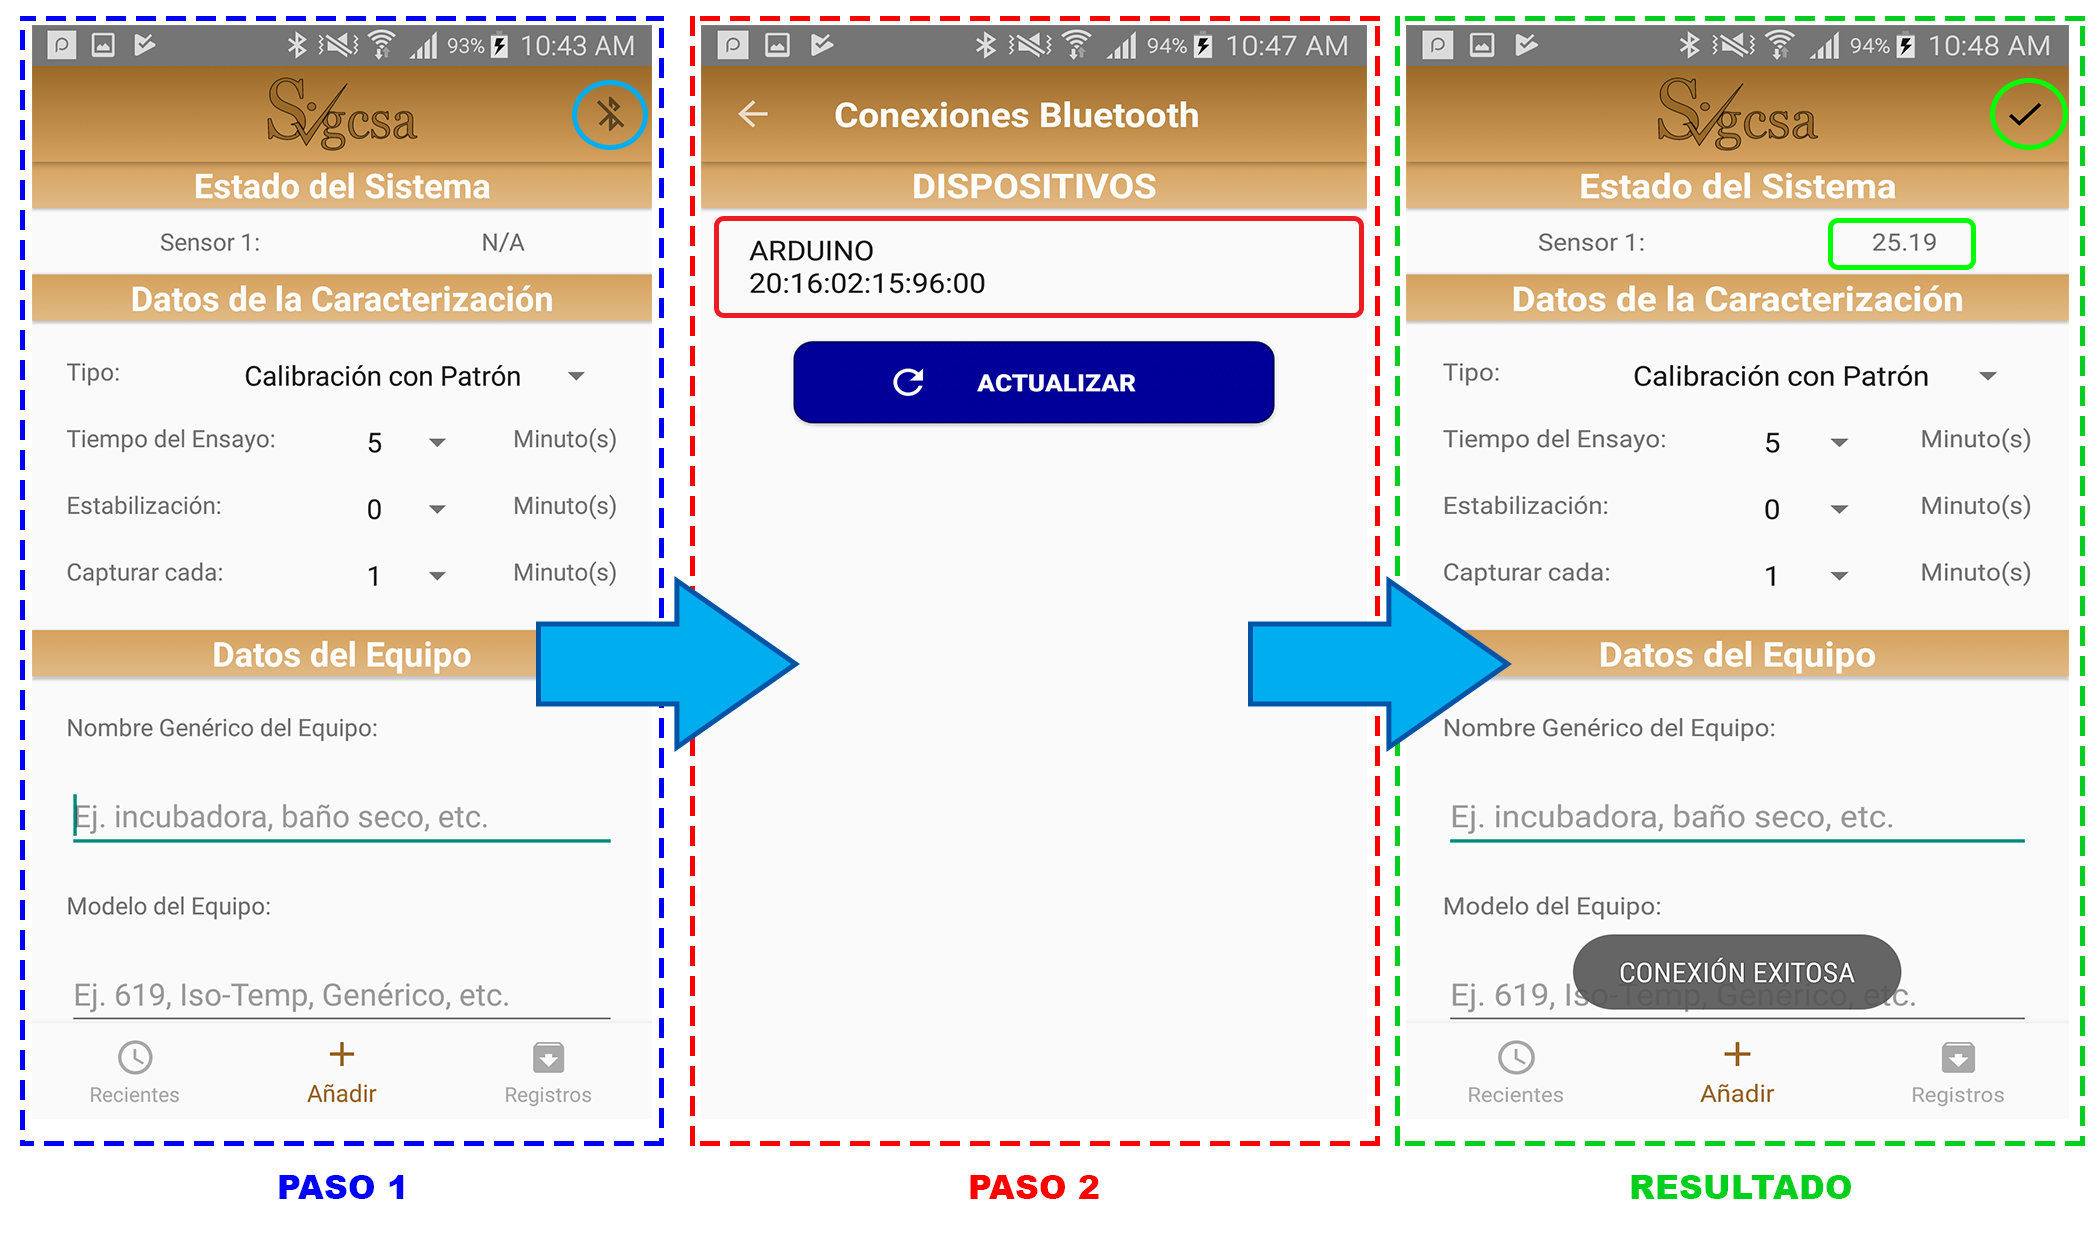
\includegraphics[width=0.8\linewidth]{interfaz13.png}
	\caption{Pasos para establecer conexión con el prototipo}
\end{figure}

\par \noindent
Si después de haber realizado una conexión con el prototipo, la conexión se pierde se enviará un mensaje al usuario indicando lo sucedido.

\begin{figure}[H]
	\centering
	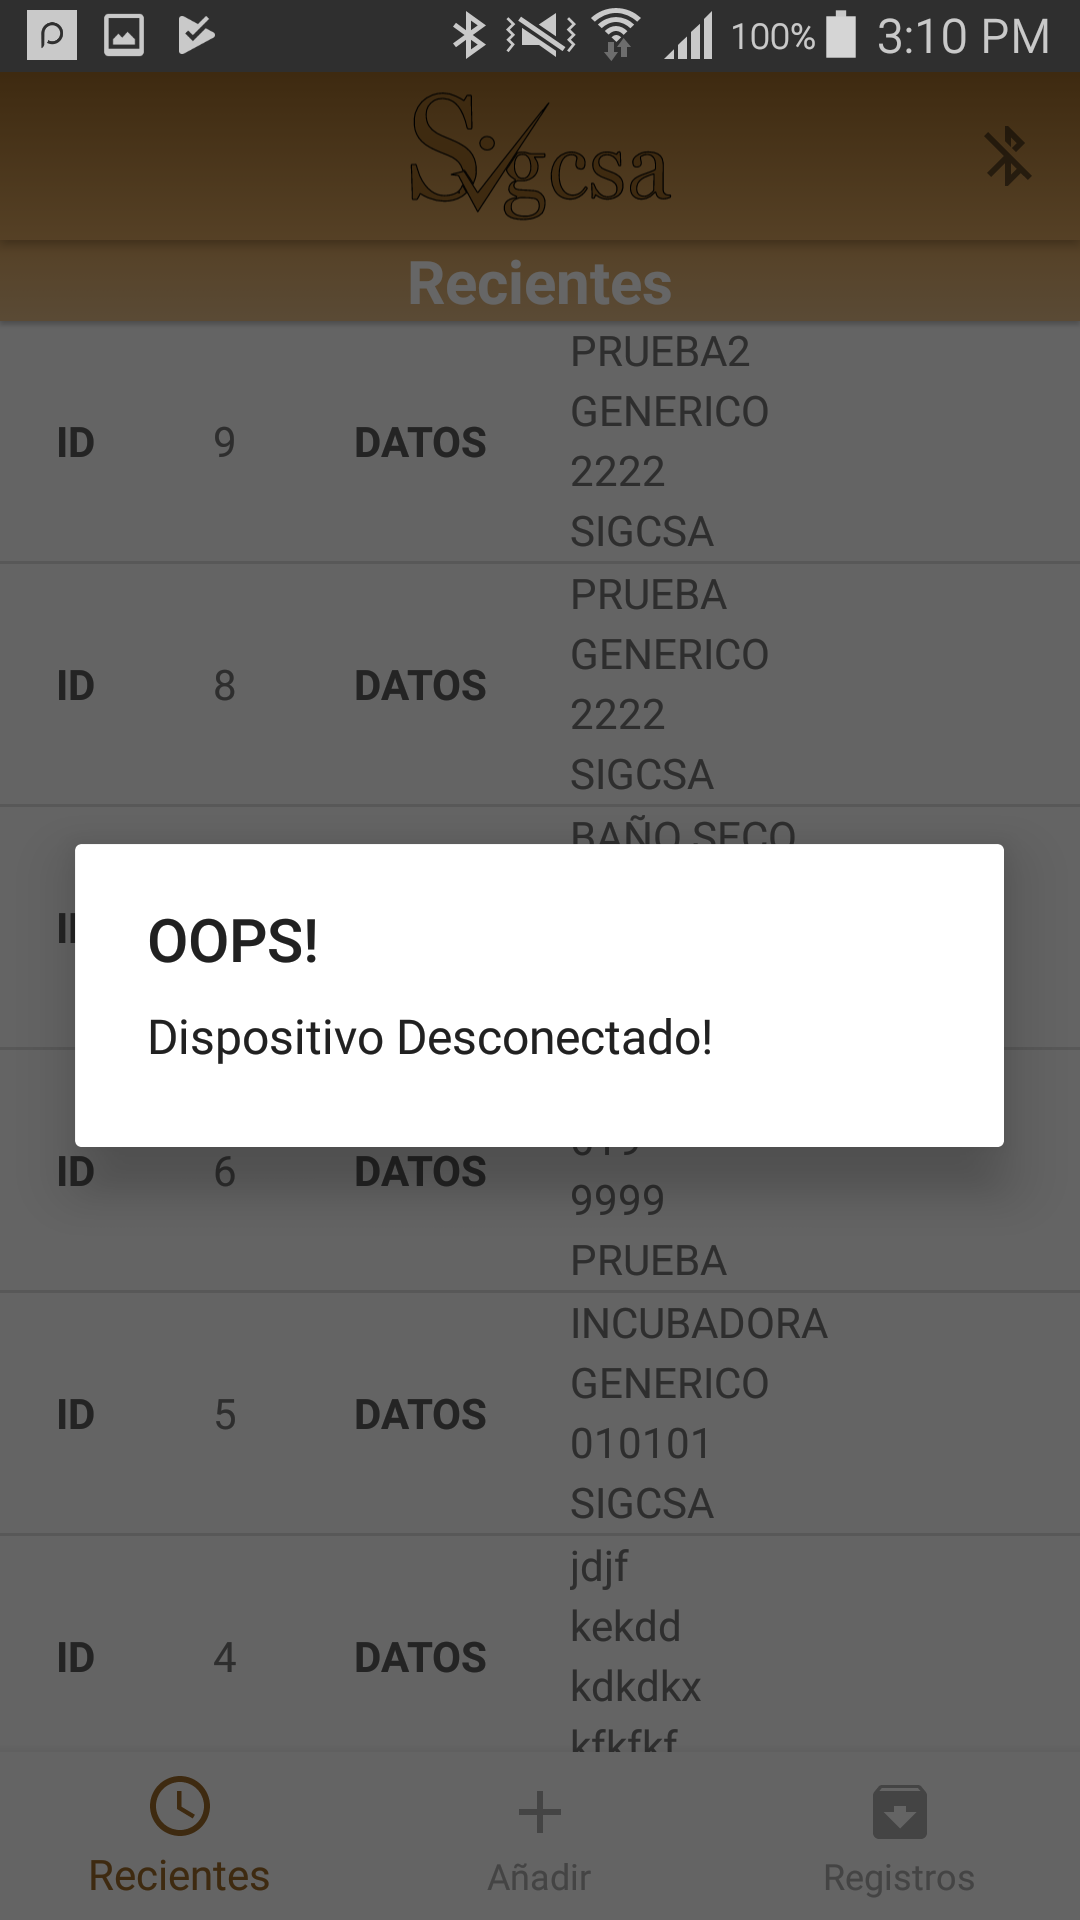
\includegraphics[width=0.3\linewidth]{interfaz14.png}
	\caption{Mensaje enviado al usuario por perdida de conexión con el prototipo}
\end{figure}

\par \noindent
Una vez hayamos establecido una conexión con nuestro prototipo podemos agregar un nuevo ensayo o medición.

\subsubsection{Agregar Nuevas Mediciones}

\par 
El agregar nuevas mediciones de temperaturas y almacenarlas en una base de datos es fundamental para nuestro proyecto. Primero debemos ubicarnos en el fragmento añadir, menú inferior de la actividad principal botón "Añadir", la aplicación debe verse como en la imagen 3.14. procedemos a seleccionar el tipo de ensayo a realizar, el tiempo del ensayo, el tiempo de estabilización y el tiempo de captura. Seguido se encuentran campos de texto para ingresar los datos del equipo a realizar el ensayo, estos campos son de texto libre. Si hemos llenado todos los campos de texto correspondientes y tenemos una comunicación activa con nuestro prototipo, el botón "INICIAR ENSAYO" se habilitará y cambiará a un color verde. Si hemos llenado los campos de texto; pero, no hemos establecido una conexión con el prototipo el botón "INICIAR ENSAYO" no se habilitará. Ocurrirá lo mismo si hemos establecido una conexión con el prototipo pero no hemos llenado los campos de texto del equipo.

\begin{figure}[H]
	\centering
	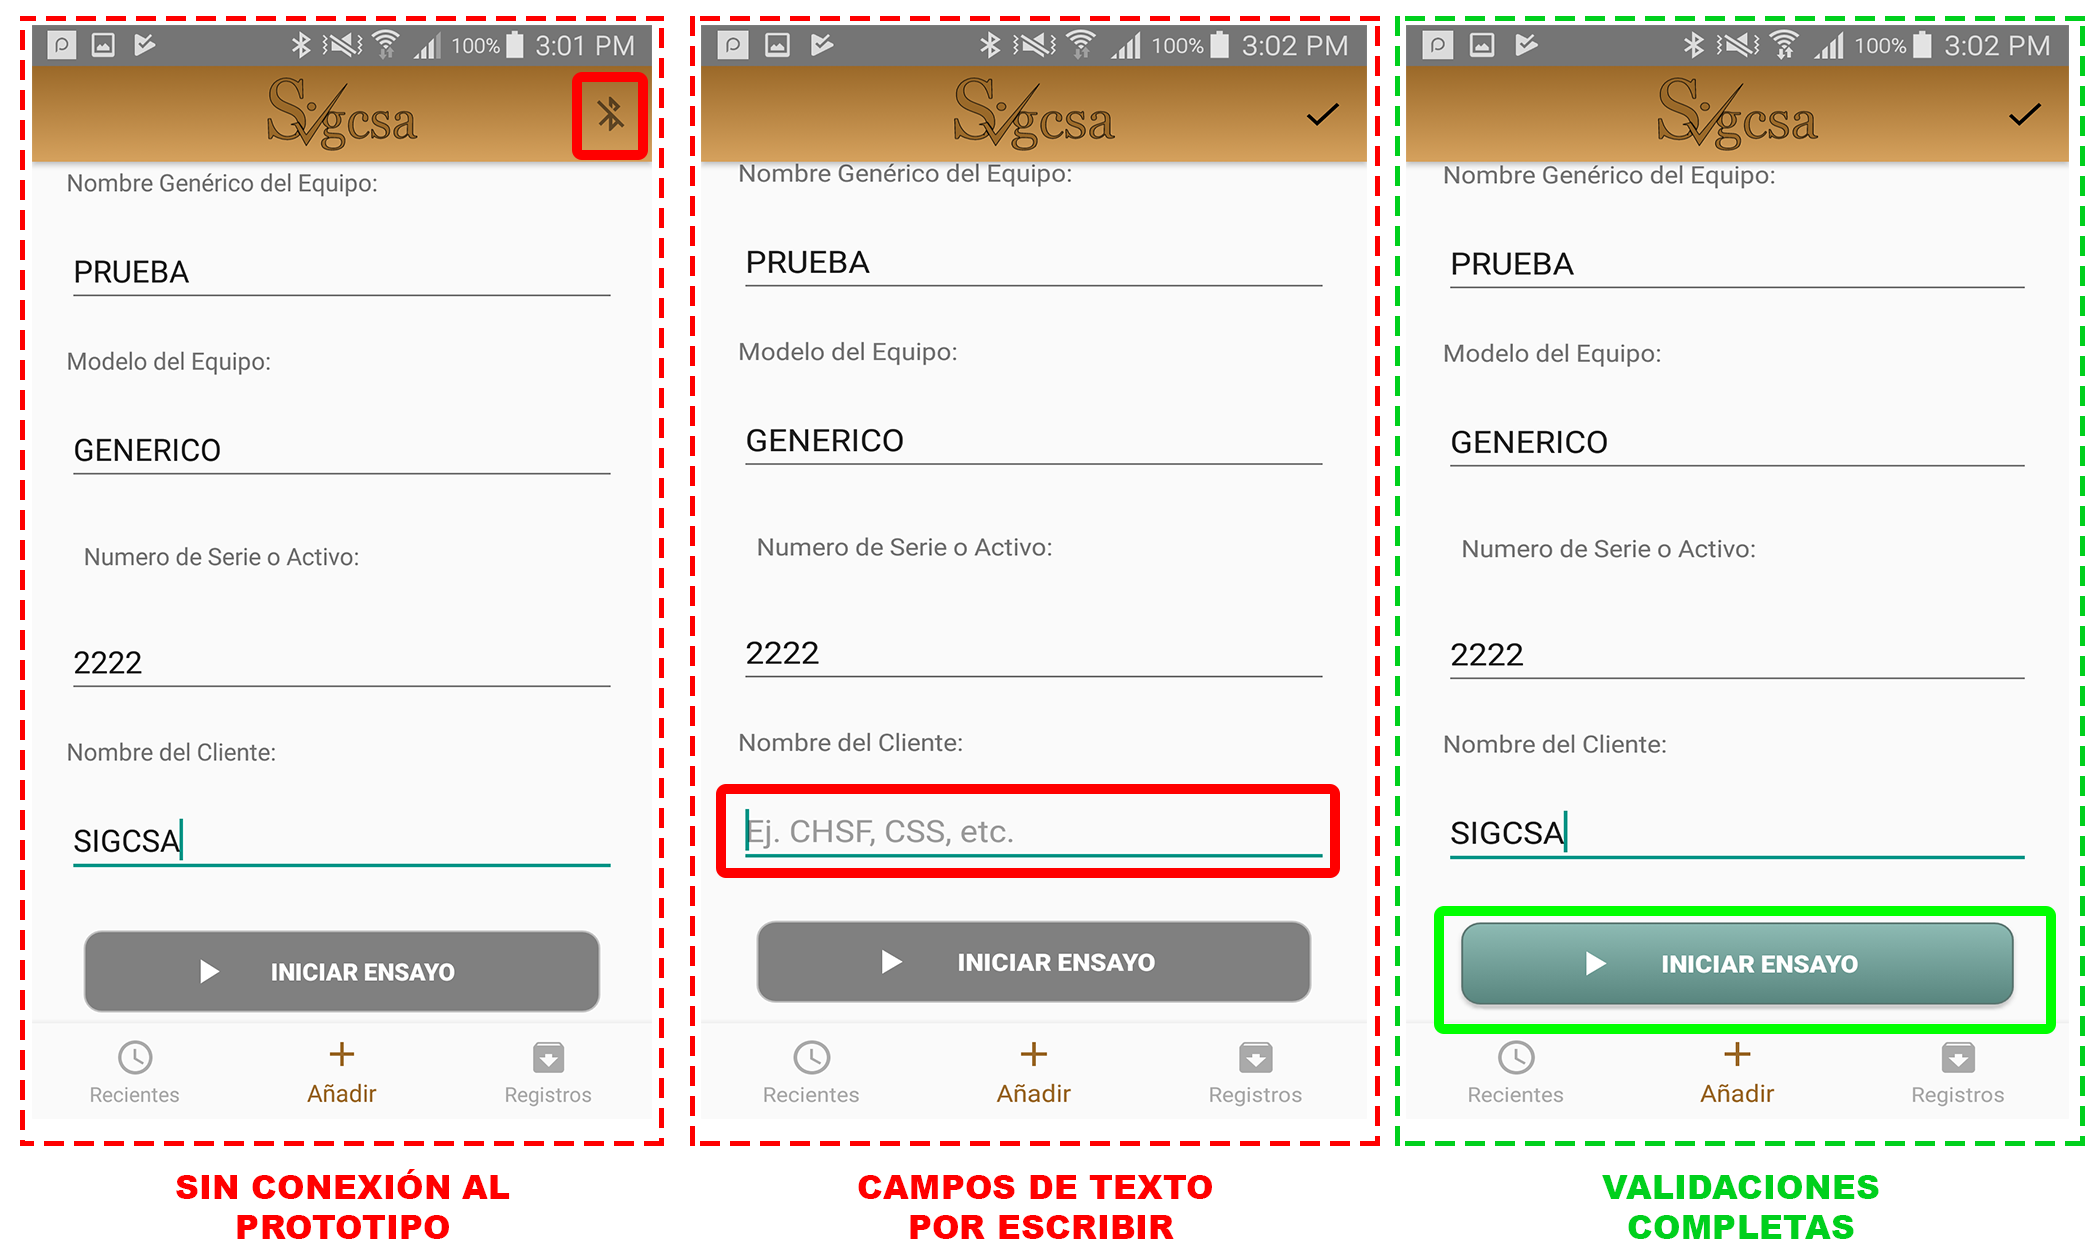
\includegraphics[width=\linewidth]{interfaz15.png}
	\caption{Validación Antes de Iniciar un Nuevo Ensayo}
\end{figure}

\par \noindent 
Una vez pulsado el botón "INICIAR ENSAYO", se deshabilitará el botón "INICIAR ENSAYO" y se habilitará el botón "CANCELAR". Además los parámetros de la medición se deshabilitarán para evitar cambios. Lo más importante es que inicia el servicio registros de mediciones el cual es el encargado de capturar los valores de los prototipos e insertarlos en la base de datos de la aplicación siguiendo los parámetros establecidos al inicio. 

\begin{figure}[H]
	\centering
	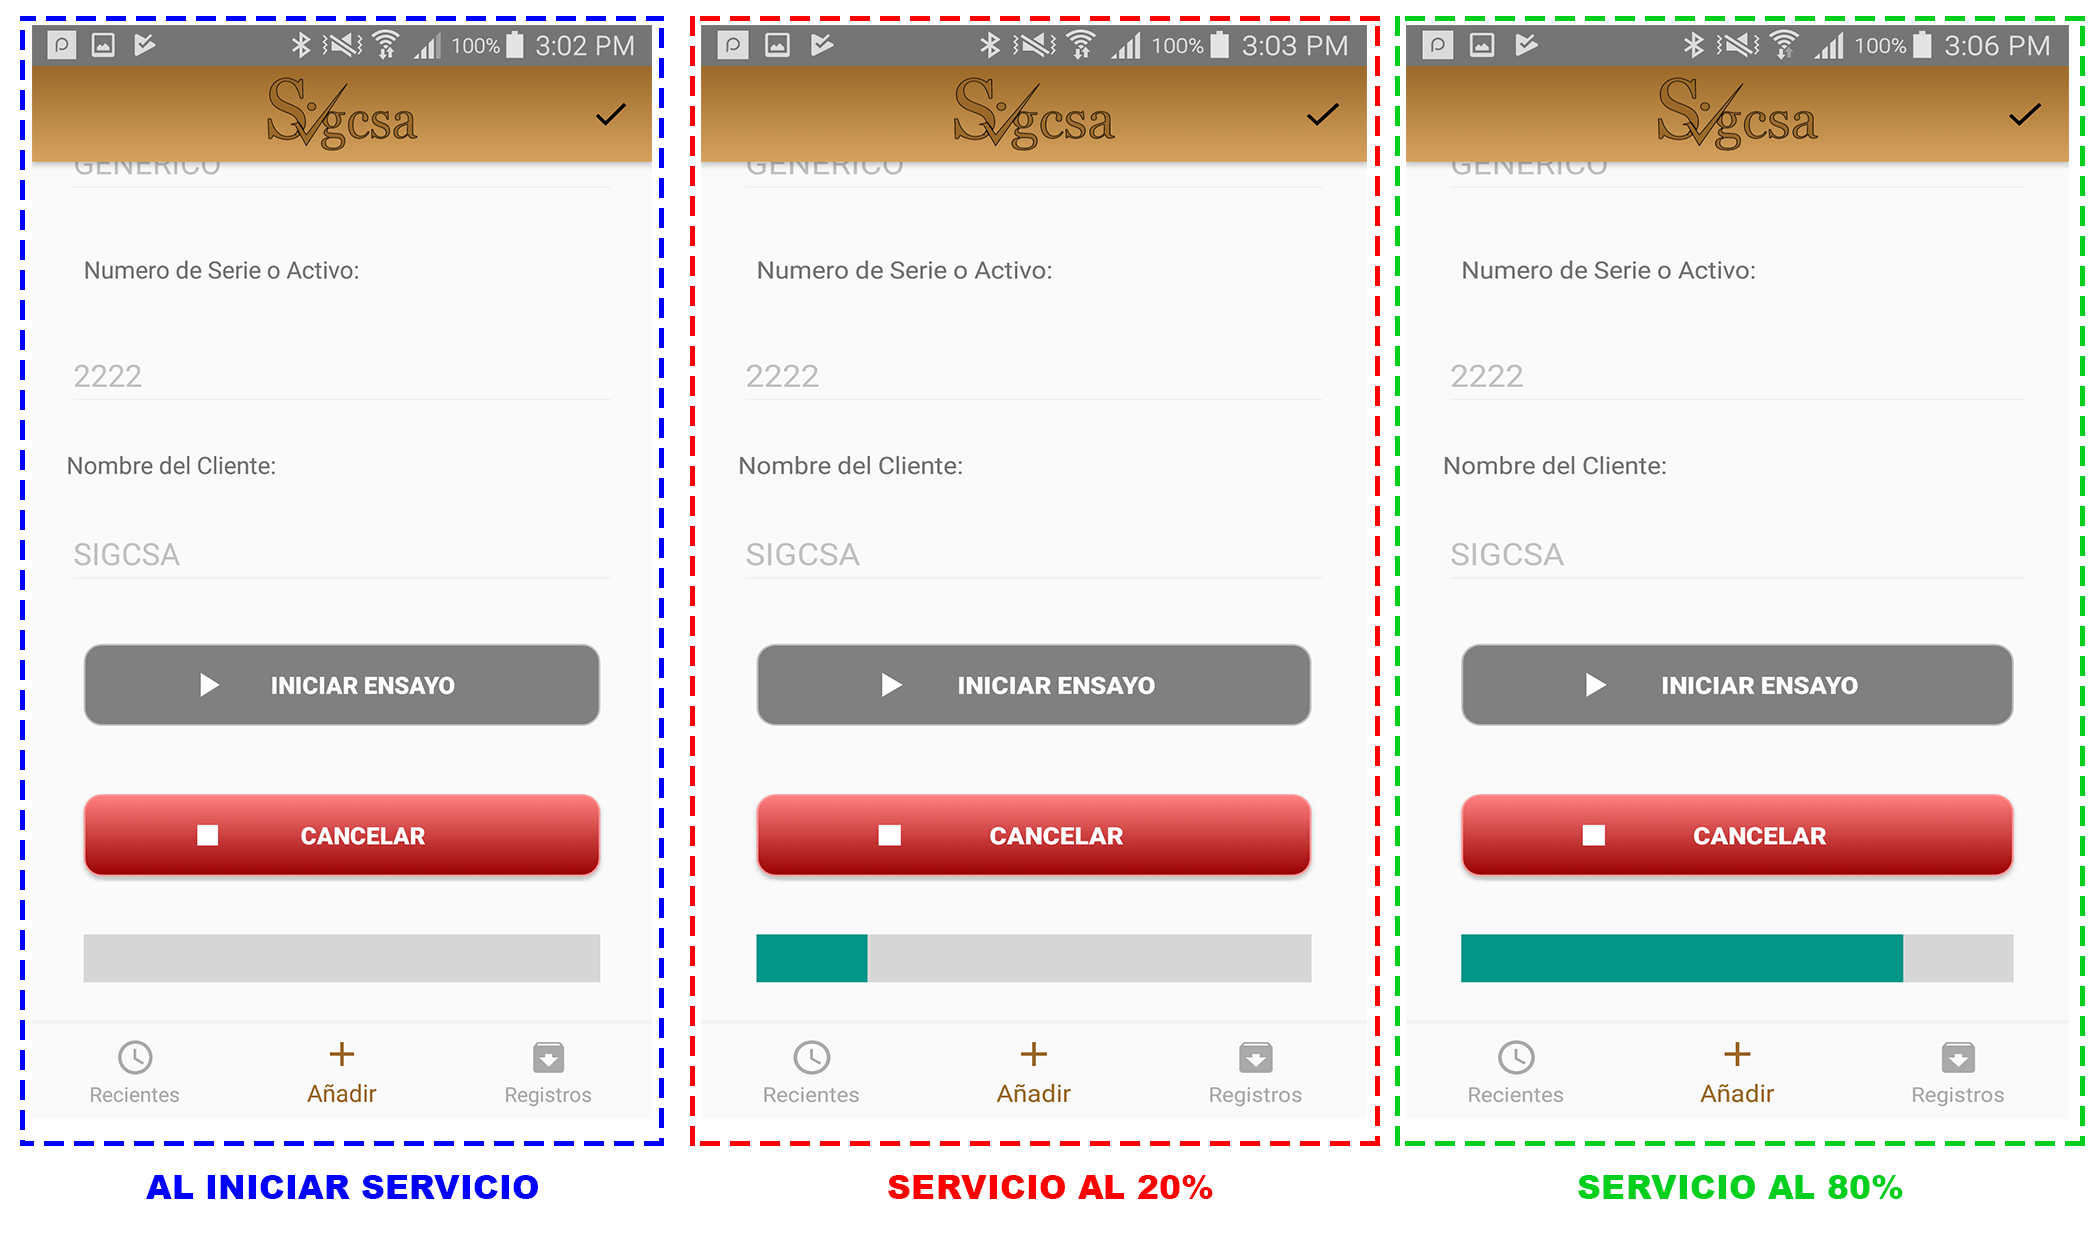
\includegraphics[width=\linewidth]{interfaz16.png}
	\caption{Proceso una vez pulsado el botón "INICIAR ENSAYO"}
\end{figure}
 
\par \noindent
Si el botón "CANCELAR" es pulsado es enviado un mensaje al servicio registros de mediciones para detener el proceso. Los valores como campos de texto y selecciones se vuelven a habilitar y el "progressbar" es reiniciado. Una vez iniciado el servicio registros de mediciones, pulsado el botón "INICIAR SERVICIO" automáticamente se graba un registro en la base de datos. Si el servicio es finalizado correctamente los valores de los campos de texto se limpian y queda el registro como "COMPLETADO" en la base de datos. 

\par \noindent
Otro punto importante es que como el servicio registro de mediciones y servicio bluetooth de la aplicación se ejecutan en segundo plano esto quiere decir que mientras la aplicación no sea borrada de memoria. Se puede ir a otra aplicación como por ejemplo: WhatsApp, Correo, YouTube, etc. y el servicio se seguirá ejecutando. Para el servicio registro de mediciones se ejecutará según desee el usuario 5 minutos o una hora; mientras que, el servicio de bluetooth se ejecuta hasta que se pierda conexión del dispositivo o que se deshabilite el bluetooth del smartphone.

\par \noindent
Una vez hayamos registrado un ensayo queremos asegurarnos de que la base de datos se haya actualizado correctamente; para poder consultar las mediciones de temperatura posteriormente.

\subsubsection{Consultar una Medición Realizada Recientemente}

\par 
Para consultar una medición realizada recientemente basta solo con ubicarse en la actividad principal y seleccionar el botón "Recientes". Cada vez que regresemos al fragmento recientes, se consulta a la base de datos de la aplicación y se retornan los últimas 10 mediciones o ensayos realizados por nuestro smartphone. La aplicación debe verse como en la imagen 3.11 donde podemos encontrar una lista de mediciones cada una con su respectiva información y número de registro (ID). Al seleccionar un elemento de la lista se desplegará más información de la medición como en la imagen 3.19. En ella se podrán acceder a las mediciones de temperatura de cada sonda de manera individual con sus respectivas características como en la imagen 3.20.

\begin{figure}[H]
	\centering
	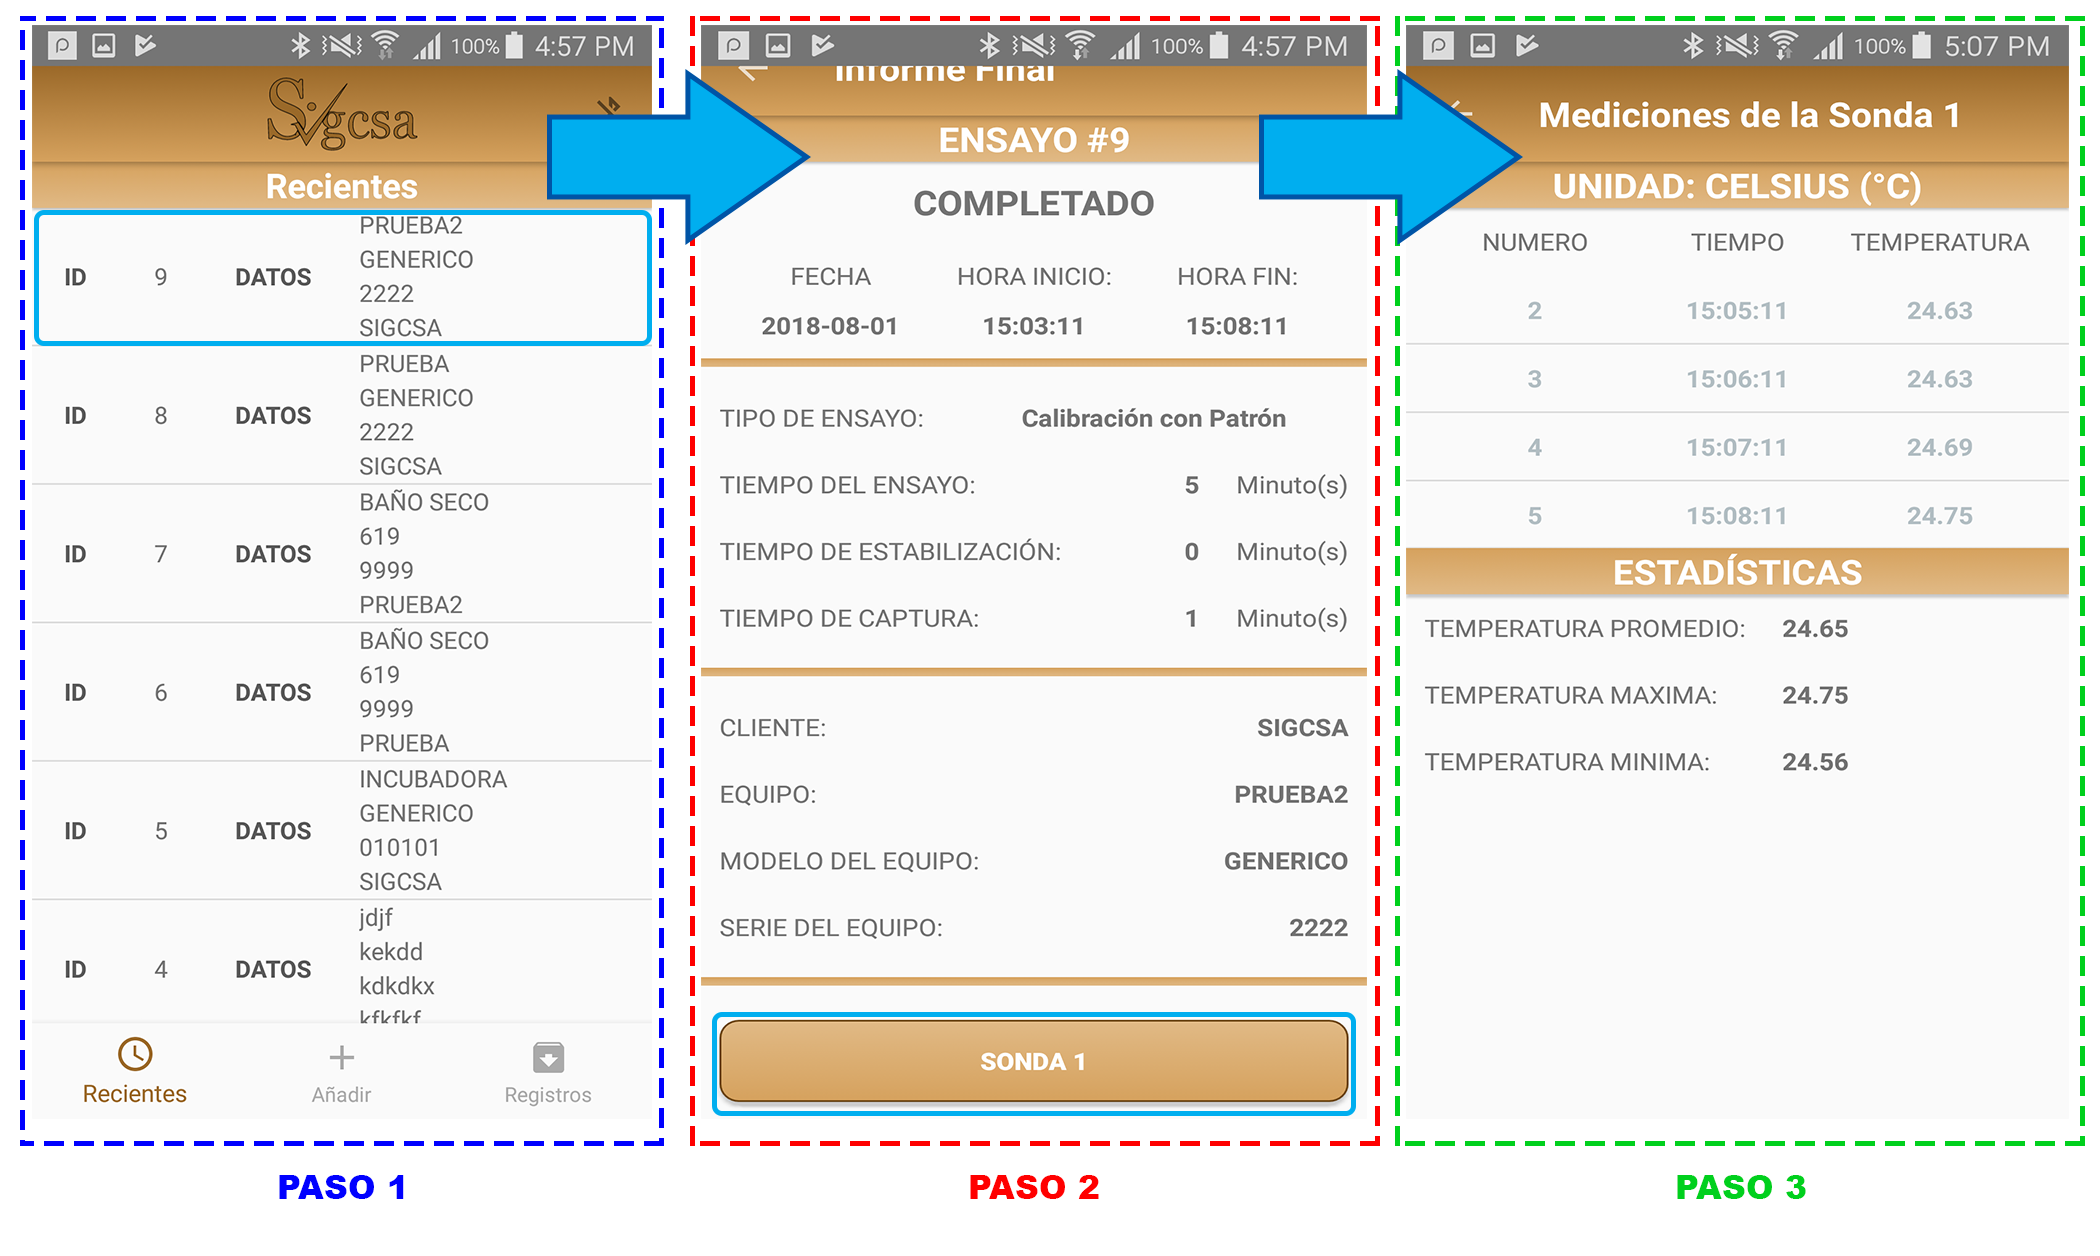
\includegraphics[width=\linewidth]{interfaz17.png}
	\caption{Proceso para consultar temperatura de una respectiva sonda en un ensayo}
\end{figure}

\par \noindent
Recordemos que siempre es posible regresar al paso anterior sea utilizando el botón en la esquina superior izquierda o utilizando la tecla de regreso del smartphone. Por último que hay si queremos consultar un ensayo en un intervalo de fechas predeterminado. 

\clearpage

\subsubsection{Consultar una Medición Realizada en una Fecha Específica}

\par 
Para consultar una medición o ensayo de una fecha específica o en un intervalo de fecha solamente hay que ubicarse en el fragmento registros, actividad principal seleccionar botón registros. La aplicación debe verse como en la imagen 3.16. Al seleccionar uno de los campos con el texto "N/A" seleccionamos las fechas deseadas, uno es para la fecha inicio la otra es para la fecha fin y seleccionamos el botón buscar. De encontrase resultados se desplegarán en un formato de lista idéntico al formato del fragmento recientes y el proceso para consultar la información es igual al proceso anterior.

\begin{figure}[H]
	\centering
	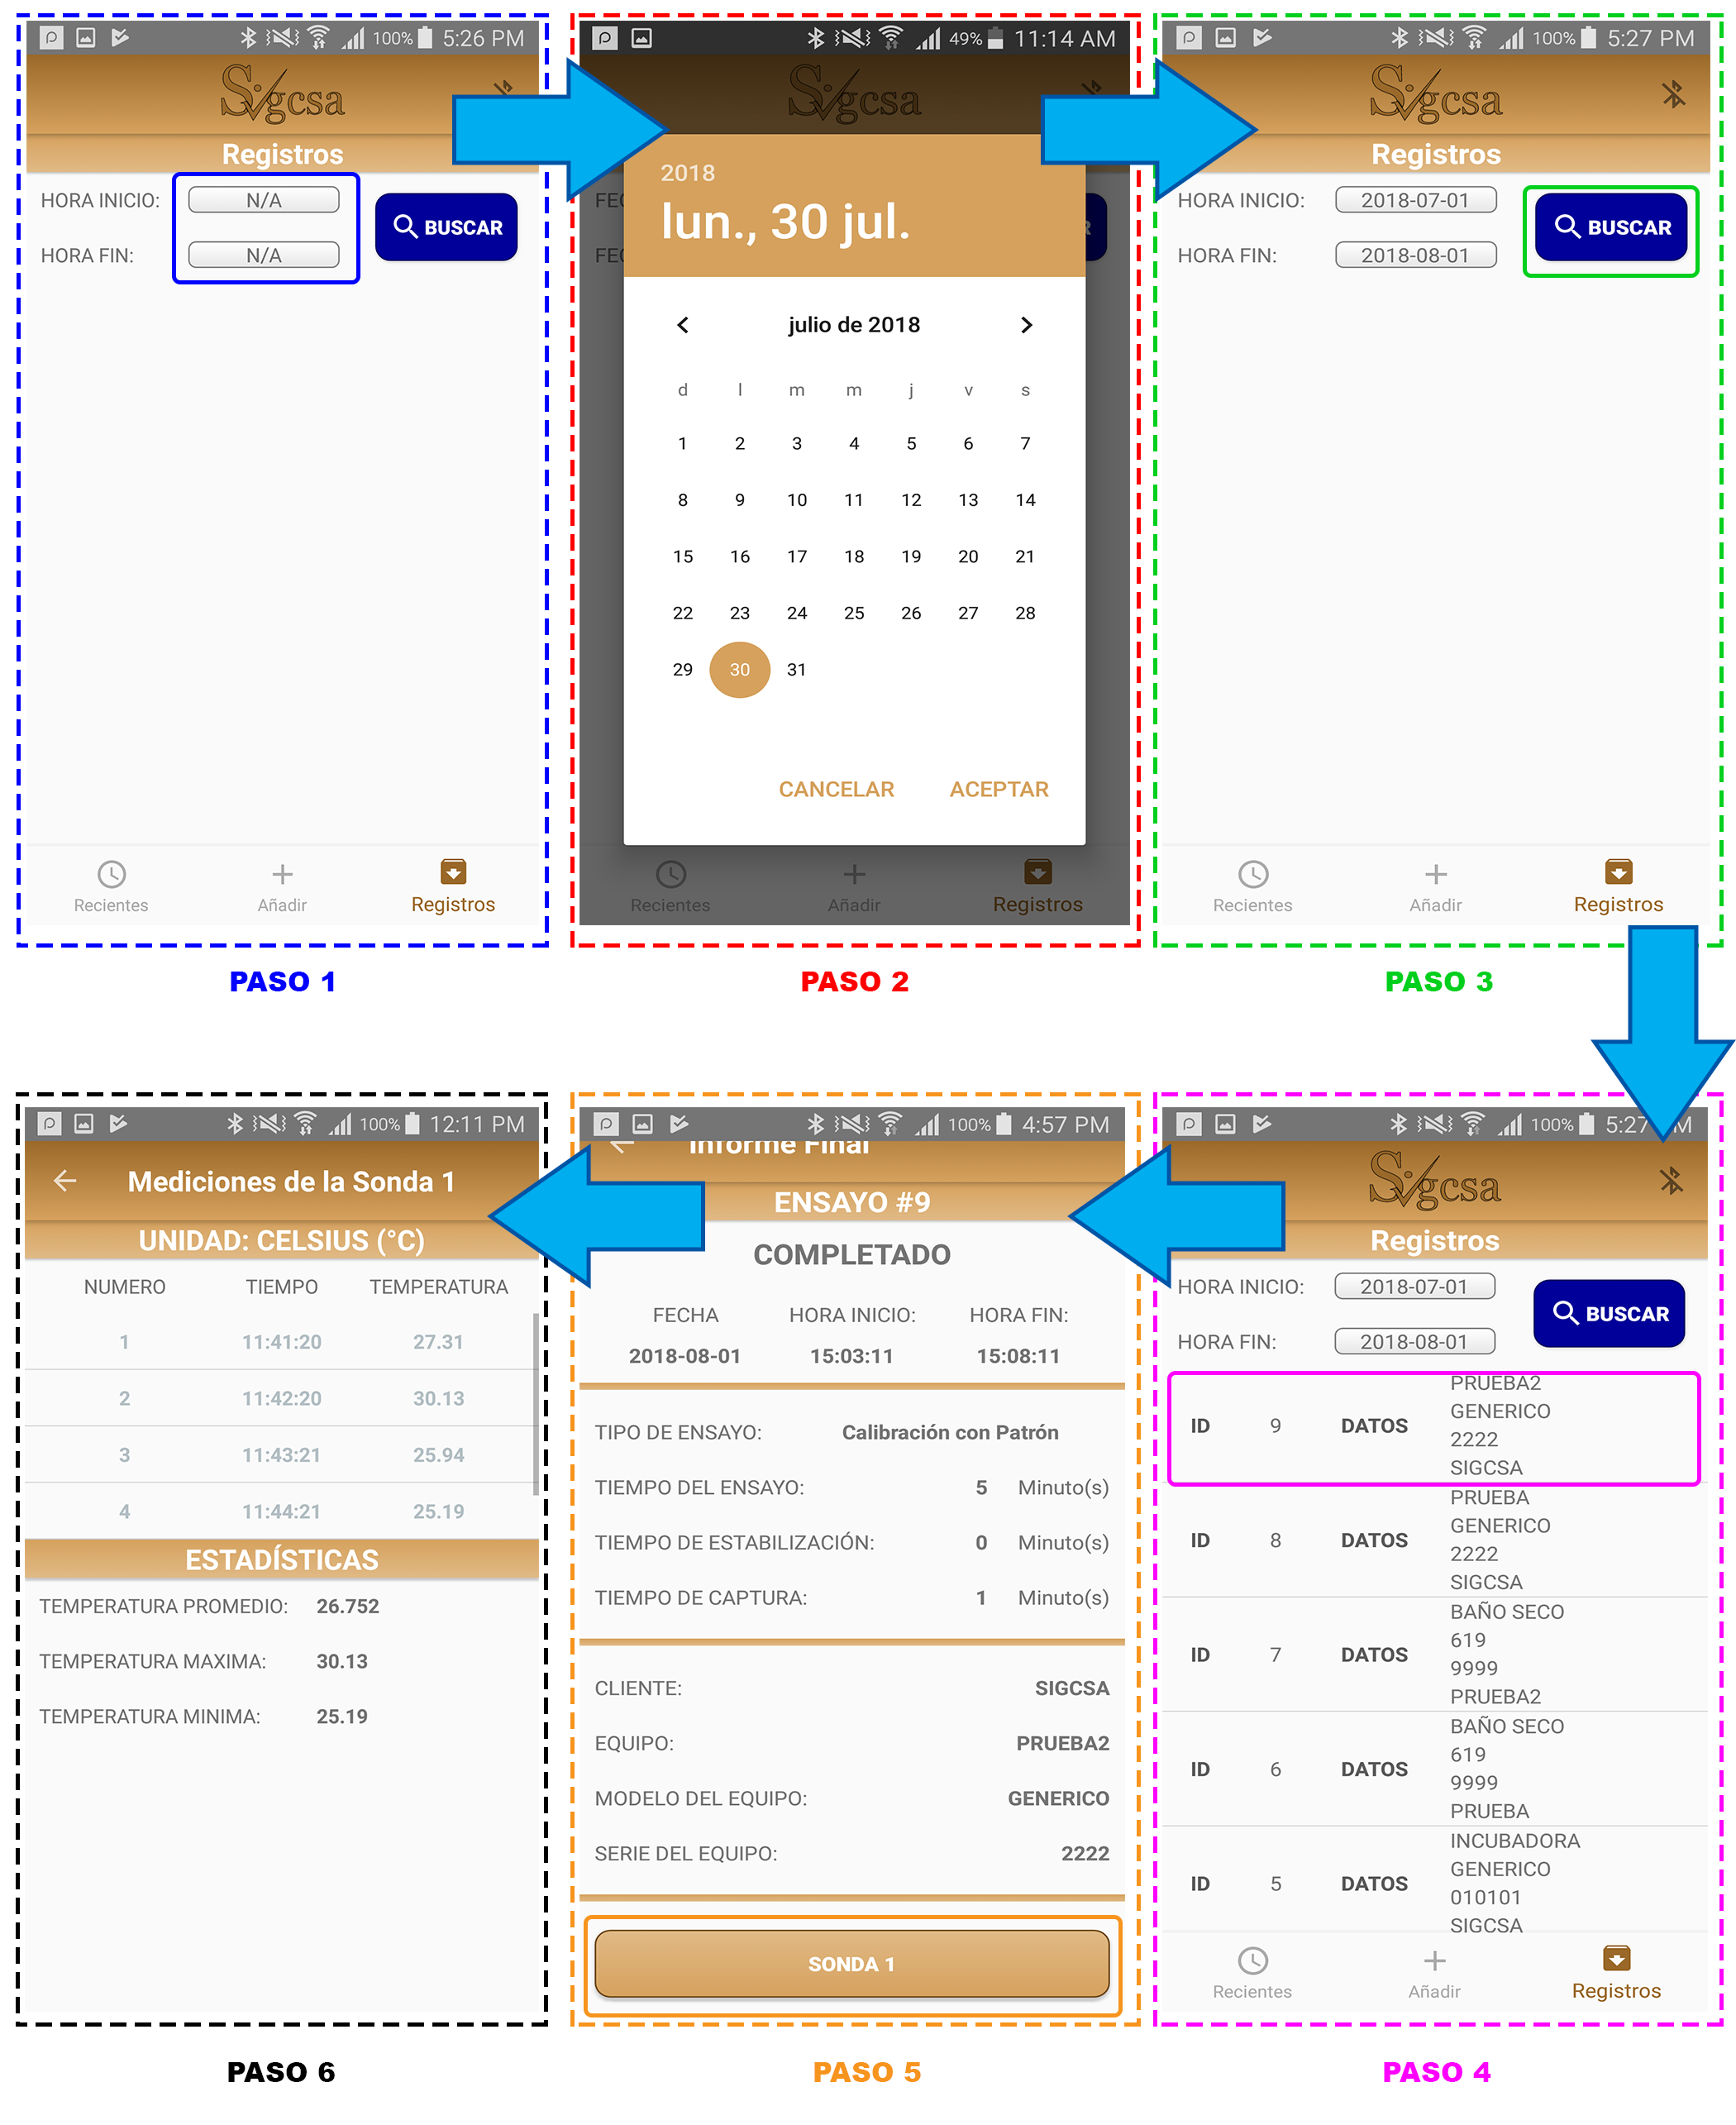
\includegraphics[width=0.8\linewidth]{interfaz18.png}
	\caption{Proceso para consultar temperatura de una respectiva sonda en un ensayo en un intervalo de fechas}
\end{figure}

\par \noindent
Ya conocemos las interfaces que se encuentran en nuestra aplicación y como utilizar en si la aplicación; sin embargo, no sabemos la parte técnica de la aplicación. Al presionar ciertos botones hacemos llamadas a servicios que se ejecutaran en el segundo plano. ¿Como funcionan estos servicios?
